%% uncomment to list all files in log
%\listfiles

\documentclass[12pt]{report}


\usepackage{fontspec}

%\setmainfont[Scale=MatchLowercase]{Lucida Bright}
%\setmonofont{FreeMono}
%\setmonofont{Source Code Pro}
\setmonofont[Scale=MatchLowercase]{Ubuntu Mono}

\usepackage[headings]{fullpage}

% national use characters 
%\usepackage{inputenc}

% ams mathematical symbols
\usepackage{amsmath,amssymb}

% added to support pandoc highlighting
\usepackage{microtype}

\usepackage{makeidx}

% add index and bibliographies to table of contents
\usepackage[nottoc]{tocbibind}

% postscript courier and times in place of cm fonts
%\usepackage{courier}
%\usepackage{times}

% extended coloring
\usepackage{color}
\usepackage[table,dvipsnames]{xcolor}
\usepackage{colortbl}

% advanced date formating
\usepackage{datetime}

%support pandoc code highlighting
\usepackage{fancyvrb}
\DefineShortVerb[commandchars=\\\{\}]{\|}
\DefineVerbatimEnvironment{Highlighting}{Verbatim}{commandchars=\\\{\}}
% Add ',fontsize=\small' for more characters per line

%tango style colors
% \usepackage{framed}
% \definecolor{shadecolor}{RGB}{255,255,255}
% \newenvironment{Shaded}{\begin{snugshade}}{\end{snugshade}}
% \newcommand{\KeywordTok}[1]{\textcolor[rgb]{0.13,0.29,0.53}{\textbf{{#1}}}}
% \newcommand{\DataTypeTok}[1]{\textcolor[rgb]{0.13,0.29,0.53}{{#1}}}
% \newcommand{\DecValTok}[1]{\textcolor[rgb]{0.00,0.00,0.81}{{#1}}}
% \newcommand{\BaseNTok}[1]{\textcolor[rgb]{0.00,0.00,0.81}{{#1}}}
% \newcommand{\FloatTok}[1]{\textcolor[rgb]{0.00,0.00,0.81}{{#1}}}
% \newcommand{\CharTok}[1]{\textcolor[rgb]{0.31,0.60,0.02}{{#1}}}
% \newcommand{\StringTok}[1]{\textcolor[rgb]{0.31,0.60,0.02}{{#1}}}
% \newcommand{\CommentTok}[1]{\textcolor[rgb]{0.56,0.35,0.01}{\textit{{#1}}}}
% \newcommand{\OtherTok}[1]{\textcolor[rgb]{0.56,0.35,0.01}{{#1}}}
% \newcommand{\AlertTok}[1]{\textcolor[rgb]{0.94,0.16,0.16}{{#1}}}
% \newcommand{\FunctionTok}[1]{\textcolor[rgb]{0.00,0.00,0.00}{{#1}}}
% \newcommand{\RegionMarkerTok}[1]{{#1}}
% \newcommand{\ErrorTok}[1]{\textbf{{#1}}}
% \newcommand{\NormalTok}[1]{{#1}}

%espresso style colors
% \usepackage{framed}
% \definecolor{shadecolor}{RGB}{42,33,28}
% \newenvironment{Shaded}{\begin{snugshade}}{\end{snugshade}}
% \newcommand{\KeywordTok}[1]{\textcolor[rgb]{0.26,0.66,0.93}{\textbf{{#1}}}}
% \newcommand{\DataTypeTok}[1]{\textcolor[rgb]{0.74,0.68,0.62}{\underline{{#1}}}}
% \newcommand{\DecValTok}[1]{\textcolor[rgb]{0.27,0.67,0.26}{{#1}}}
% \newcommand{\BaseNTok}[1]{\textcolor[rgb]{0.27,0.67,0.26}{{#1}}}
% \newcommand{\FloatTok}[1]{\textcolor[rgb]{0.27,0.67,0.26}{{#1}}}
% \newcommand{\CharTok}[1]{\textcolor[rgb]{0.02,0.61,0.04}{{#1}}}
% \newcommand{\StringTok}[1]{\textcolor[rgb]{0.02,0.61,0.04}{{#1}}}
% \newcommand{\CommentTok}[1]{\textcolor[rgb]{0.00,0.40,1.00}{\textit{{#1}}}}
% \newcommand{\OtherTok}[1]{\textcolor[rgb]{0.74,0.68,0.62}{{#1}}}
% \newcommand{\AlertTok}[1]{\textcolor[rgb]{1.00,1.00,0.00}{{#1}}}
% \newcommand{\FunctionTok}[1]{\textcolor[rgb]{1.00,0.58,0.35}{\textbf{{#1}}}}
% \newcommand{\RegionMarkerTok}[1]{\textcolor[rgb]{0.74,0.68,0.62}{{#1}}}
% \newcommand{\ErrorTok}[1]{\textcolor[rgb]{0.74,0.68,0.62}{\textbf{{#1}}}}
% \newcommand{\NormalTok}[1]{\textcolor[rgb]{0.74,0.68,0.62}{{#1}}}

%kete style colors
% \newenvironment{Shaded}{}{}
% \newcommand{\KeywordTok}[1]{\textbf{{#1}}}
% \newcommand{\DataTypeTok}[1]{\textcolor[rgb]{0.50,0.00,0.00}{{#1}}}
% \newcommand{\DecValTok}[1]{\textcolor[rgb]{0.00,0.00,1.00}{{#1}}}
% \newcommand{\BaseNTok}[1]{\textcolor[rgb]{0.00,0.00,1.00}{{#1}}}
% \newcommand{\FloatTok}[1]{\textcolor[rgb]{0.50,0.00,0.50}{{#1}}}
% \newcommand{\CharTok}[1]{\textcolor[rgb]{1.00,0.00,1.00}{{#1}}}
% \newcommand{\StringTok}[1]{\textcolor[rgb]{0.87,0.00,0.00}{{#1}}}
% \newcommand{\CommentTok}[1]{\textcolor[rgb]{0.50,0.50,0.50}{\textit{{#1}}}}
% \newcommand{\OtherTok}[1]{{#1}}
% \newcommand{\AlertTok}[1]{\textcolor[rgb]{0.00,1.00,0.00}{\textbf{{#1}}}}
% \newcommand{\FunctionTok}[1]{\textcolor[rgb]{0.00,0.00,0.50}{{#1}}}
% \newcommand{\RegionMarkerTok}[1]{{#1}}
% \newcommand{\ErrorTok}[1]{\textcolor[rgb]{1.00,0.00,0.00}{\textbf{{#1}}}}
% \newcommand{\NormalTok}[1]{{#1}}
%end pandoc code hacks

% jodliterate colors
\usepackage{color}
\definecolor{shadecolor}{RGB}{248,248,248}
% j control structures 
\definecolor{keywcolor}{rgb}{0.13,0.29,0.53}
% j explicit arguments x y m n u v
\definecolor{datacolor}{rgb}{0.13,0.29,0.53}
% j numbers - all types see j.xml
\definecolor{decvcolor}{rgb}{0.00,0.00,0.81}
\definecolor{basencolor}{rgb}{0.00,0.00,0.81}
\definecolor{floatcolor}{rgb}{0.00,0.00,0.81}
% j local assignments
\definecolor{charcolor}{rgb}{0.31,0.60,0.02}
\definecolor{stringcolor}{rgb}{0.31,0.60,0.02}
\definecolor{commentcolor}{rgb}{0.56,0.35,0.01}
% primitive adverbs and conjunctions
%\definecolor{othercolor}{rgb}{0.56,0.35,0.01}   
\definecolor{othercolor}{RGB}{0,0,255}
% global assignments
\definecolor{alertcolor}{rgb}{0.94,0.16,0.16}
% primitive J verbs and noun names
\definecolor{funccolor}{rgb}{0.00,0.00,0.00}    

\usepackage{framed}
\newenvironment{Shaded}{}{}
\newcommand{\KeywordTok}[1]{\textcolor{keywcolor}{\textbf{{#1}}}}
\newcommand{\DataTypeTok}[1]{\textcolor{datacolor}{{#1}}}
%\newcommand{\DecValTok}[1]{\textcolor{decvcolor}{{#1}}}
\newcommand{\DecValTok}[1]{{#1}} 
\newcommand{\BaseNTok}[1]{\textcolor{basencolor}{{#1}}}
\newcommand{\FloatTok}[1]{\textcolor{floatcolor}{{#1}}}
\newcommand{\CharTok}[1]{\textcolor{charcolor}{\textbf{{#1}}}}
\newcommand{\StringTok}[1]{\textcolor{stringcolor}{{#1}}}
\newcommand{\CommentTok}[1]{\textcolor{commentcolor}{\textit{{#1}}}}
\newcommand{\OtherTok}[1]{\textcolor{othercolor}{{#1}}} 
\newcommand{\AlertTok}[1]{\textcolor{alertcolor}{\textbf{{#1}}}}
%\newcommand{\FunctionTok}[1]{\textcolor{funccolor}{{#1}}}
\newcommand{\FunctionTok}[1]{{#1}}
\newcommand{\RegionMarkerTok}[1]{{#1}}
\newcommand{\ErrorTok}[1]{\textbf{{#1}}}
\newcommand{\NormalTok}[1]{{#1}}

% headers and footers
\usepackage{fancyhdr}
\pagestyle{fancy}

\fancyhead{}
\fancyfoot{}

%\fancyhead[LE,RO]{\slshape \rightmark}
%\fancyhead[LO,RE]{\slshape \leftmark}
\fancyfoot[C]{\thepage}
%\headrulewidth 0.4pt
%\footrulewidth 0 pt

%\addtolength{\headheight}{\baselineskip}

%\lfoot{\emph{Analyze the Data not the Drivel}}
%\rfoot{\emph{\today}}

% subfigure handles figures that contain subfigures
%\usepackage{color,graphicx,subfigure,sidecap}
\usepackage{graphicx,sidecap}
\usepackage{subfigure}
\graphicspath{{./inclusions/}}

% floatflt provides for text wrapping around small figures and tables
\usepackage{floatflt}

% tweak caption formats 
\usepackage{caption} 
\usepackage{sidecap}
%\usepackage{subcaption} % not compatible with subfigure

\usepackage{rotating} % flip tables sideways

% complex footnotes
%\usepackage{bigfoot}

% weird logos \XeLaTeX
\usepackage{metalogo}

% source code listings
\usepackage{listings}

% long tables
% \usepackage{longtable}

\newcommand{\HRule}{\rule{\linewidth}{0.5mm}}

% map LaTeX cross references into PDF cross references
\usepackage[
            %dvips,
            colorlinks,
            linkcolor=blue,
            citecolor=blue,
            urlcolor=blue,   % magenta, cyan default        
            pdfauthor={John D. Baker},
            pdftitle={Analyze the Data not the Drivel},
            pdfsubject={Blog},
            pdfcreator={MikTeX+LaTeXe with hyperref package},
            pdfkeywords={blog,wordpress},
            ]{hyperref}
           
% custom colors
\definecolor{CodeBackGround}{cmyk}{0.0,0.0,0,0.05}    % light gray
\definecolor{CodeComment}{rgb}{0,0.50,0.00}           % dark green {0,0.45,0.08}
\definecolor{TableStripes}{gray}{0.9}                 % odd/even background in tables

\lstdefinelanguage{bat}
{morekeywords={echo,title,pushd,popd,setlocal,endlocal,off,if,not,exist,set,goto,pause},
sensitive=True,
morecomment=[l]{rem}
}

\lstdefinelanguage{jdoc}
{
morekeywords={},
otherkeywords={assert.,break.,continue.,for.,do.,if.,else.,elseif.,return.,select.,end.
,while.,whilst.,throw.,catch.,catchd.,catcht.,try.,case.,fcase.},
sensitive=True,
morecomment=[l]{NB.},
morestring=[b]',
morestring=[d]',
}

% latex size ordering - can never remember it
% \tiny
% \scriptsize
% \footnotesize
% \small
% \normalsize
% \large
% \Large
% \LARGE
% \huge
% \Huge
 
% listings package settings  
\lstset{%
  language=jdoc,                                % j document settings
  basicstyle=\ttfamily\footnotesize,            
  keywordstyle=\bfseries\color{keywcolor}\footnotesize,
  identifierstyle=\color{black},
  commentstyle=\slshape\color{CodeComment},     % colored slanted comments
  stringstyle=\color{red}\ttfamily,
  showstringspaces=false,                       
  %backgroundcolor=\color{CodeBackGround},       
  frame=single,                                
  framesep=1pt,                                 
  framerule=0.8pt,                             
  rulecolor=\color{CodeBackGround},   
  showspaces=false,
  %columns=fullflexible,
  %numbers=left,
  %numberstyle=\footnotesize,
  %numbersep=9pt,
  tabsize=2,
  showtabs=false,
  captionpos=b
  breaklines=true,                              
  breakindent=5pt                              
}

\lstdefinelanguage{JavaScript}{
  keywords={typeof, new, true, false, catch, function, return, null, catch, switch, var, if, in, while, do, else, case, break},
  ndkeywords={class, export, boolean, throw, implements, import, this},
  ndkeywordstyle=\color{darkgray}\bfseries,
  sensitive=false,
  comment=[l]{//},
  morecomment=[s]{/*}{*/},
  morestring=[b]',
  morestring=[b]"
}

% C# settings
\lstdefinestyle{sharpc}{
language=[Sharp]C,
basicstyle=\ttfamily\scriptsize, 
keywordstyle=\bfseries\color{keywcolor}\scriptsize,
framerule=0pt
}

% for source code listing longer than two use smaller font
\lstdefinestyle{smallersource}{
basicstyle=\ttfamily\scriptsize, 
keywordstyle=\bfseries\color{keywcolor}\scriptsize,
framerule=0pt
}

\lstdefinestyle{resetdefaults}{
language=jdoc,
basicstyle=\ttfamily\footnotesize,  
keywordstyle=\bfseries\color{keywcolor}\footnotesize,                                                               
framerule=0.8pt 
}

% APL UTF8 code points listed for lstlisting processing
\makeatletter
\lst@InputCatcodes
\def\lst@DefEC{%
 \lst@CCECUse \lst@ProcessLetter
  ^^80^^81^^82^^83^^84^^85^^86^^87^^88^^89^^8a^^8b^^8c^^8d^^8e^^8f%
  ^^90^^91^^92^^93^^94^^95^^96^^97^^98^^99^^9a^^9b^^9c^^9d^^9e^^9f%
  ^^a0^^a1^^a2^^a3^^a4^^a5^^a6^^a7^^a8^^a9^^aa^^ab^^ac^^ad^^ae^^af%
  ^^b0^^b1^^b2^^b3^^b4^^b5^^b6^^b7^^b8^^b9^^ba^^bb^^bc^^bd^^be^^bf%
  ^^c0^^c1^^c2^^c3^^c4^^c5^^c6^^c7^^c8^^c9^^ca^^cb^^cc^^cd^^ce^^cf%
  ^^d0^^d1^^d2^^d3^^d4^^d5^^d6^^d7^^d8^^d9^^da^^db^^dc^^dd^^de^^df%
  ^^e0^^e1^^e2^^e3^^e4^^e5^^e6^^e7^^e8^^e9^^ea^^eb^^ec^^ed^^ee^^ef%
  ^^f0^^f1^^f2^^f3^^f4^^f5^^f6^^f7^^f8^^f9^^fa^^fb^^fc^^fd^^fe^^ff%
  ^^^^20ac^^^^0153^^^^0152%
  ^^^^20a7^^^^2190^^^^2191^^^^2192^^^^2193^^^^2206^^^^2207^^^^220a%
  ^^^^2218^^^^2228^^^^2229^^^^222a^^^^2235^^^^223c^^^^2260^^^^2261%
  ^^^^2262^^^^2264^^^^2265^^^^2282^^^^2283^^^^2296^^^^22a2^^^^22a3%
  ^^^^22a4^^^^22a5^^^^22c4^^^^2308^^^^230a^^^^2336^^^^2337^^^^2339%
  ^^^^233b^^^^233d^^^^233f^^^^2340^^^^2342^^^^2347^^^^2348^^^^2349%
  ^^^^234b^^^^234e^^^^2350^^^^2352^^^^2355^^^^2357^^^^2359^^^^235d%
  ^^^^235e^^^^235f^^^^2361^^^^2362^^^^2363^^^^2364^^^^2365^^^^2368%
  ^^^^236a^^^^236b^^^^236c^^^^2371^^^^2372^^^^2373^^^^2374^^^^2375%
  ^^^^2377^^^^2378^^^^237a^^^^2395^^^^25af^^^^25ca^^^^25cb%  
  ^^00}
\lst@RestoreCatcodes
\makeatother

% custom lengths used within minipages
\newcommand{\minindent}{17pt}


\makeindex

\begin{document}

\subsection*{\href{https://bakerjd99.wordpress.com/2013/01/04/my-dream-of-liberty-encased/}{My Dream of Liberty Encased}}
\addcontentsline{toc}{subsection}{My Dream of Liberty Encased}


\noindent\emph{Posted: 05 Jan 2013 05:31:35}
\vspace{6pt}

I have cinematic dreams that I watch as a little sleeping movie critic.
I'm sure you're familiar with this weird state of consciousness. You
know you're asleep and dreaming; the dream is unfolding around you, but
part of your mind, the part that knows you're dreaming, is aware and
watching. It's busy taking notes, making snide remarks, lamenting poor
production values and snickering at clichés. Sometimes it's surprised
and delighted by unexpected turns. This morning I had an entertaining
dream.

%\href{http://conceptcontrol.smugmug.com/Trips/USA-and-Canada/New-York-2005-1/7461666\_BQ3QDf\#!i=481352959\&k=thrPPpx\&lb=1\&s=A}{\includegraphics{statue%20of%20liberty%202%20%5B3962082%5D-M.jpg}}
 
I was visiting the Statue of Liberty for the second time. I've seen the
statue in my waking life and it is well worth the security shakedown
you'll get before boarding the ferry at
\href{http://www.statuecruises.com/pd\_directions.html}{Battery Park}.
In my dream I knew that many years had passed since my last visit and I
was nervous about recent changes. As the ferry pulled up to the statue's
island my concerns materialized. The entire island had been
``redeveloped.'' The little park at the base of the statue was gone:
replaced by a massive marble covered plaza. Standing in the middle of
the plaza was a large, hideous, marble, glass and steel building that
completely enclosed the statue. From the island boat dock
you couldn't even see Liberty! ``Oh crap,'' my dreaming self muttered.
Large signs on the dock warned us about ``demonstrative language.'' We
were to conduct ourselves with quiet dignity while visiting this
``shrine of democracy.'' My dreaming self, and the little sleeping movie
critic, both inwardly groaned. Nothing says ``democracy'' like shutting
up and taking whatever's doled out.

I got off the boat feeling hopeful; there had to be a good vantage point
to look at Liberty. I was carrying my cameras, so I set off exploring
the plaza looking for a good place to take pictures. The plaza was still
under construction. Construction fencing blocked off the plaza behind
the Liberty building. You couldn't walk around the building, but you
could go far enough to see that the walls were completely opaque on all
sides except the front, where Liberty gazed at the harbor. Her back and
sides were completely hidden and exceptionally thick steel girders
buttressed the back wall. ``That ought to block incoming planes,'' my
dream self thought. My little movie critic wasn't happy. \emph{Liberty
is about open possibilities in all directions.} It's not about being
stuffed in a box and hidden from view. All my selves found it
difficult to believe that some moron thought it was a good idea to
completely cover the thing we were all there to see.

Determined to get a good picture, I turned back from the construction
fence and walked along the base of the building. On the way I passed two
little men dressed in black; they were staging a puppet show. Only the
puppets weren't little dolls on strings they were massive pantomime
robots that towered over the tourists. The giant robots were exactly
mimicking what the little men were doing. My somnolent movie critic
thought, ``Cute -- the great men are really just little men putting on a
big show. If you take away their puppets they're even smaller and more
pathetic than the rest of us.'' I took a moment to congratulate my
dreaming self for abruptly injecting this metaphor while also noting it
was too blatant for refined tastes.


\captionsetup[floatingfigure]{labelformat=empty}
\begin{floatingfigure}[r]{0.27\textwidth}
\centering
\href{http://conceptcontrol.smugmug.com/Trips/USA-and-Canada/New-York-2005-1/7461666\_BQ3QDf\#!i=481352959\&k=thrPPpx\&lb=1\&s=A}{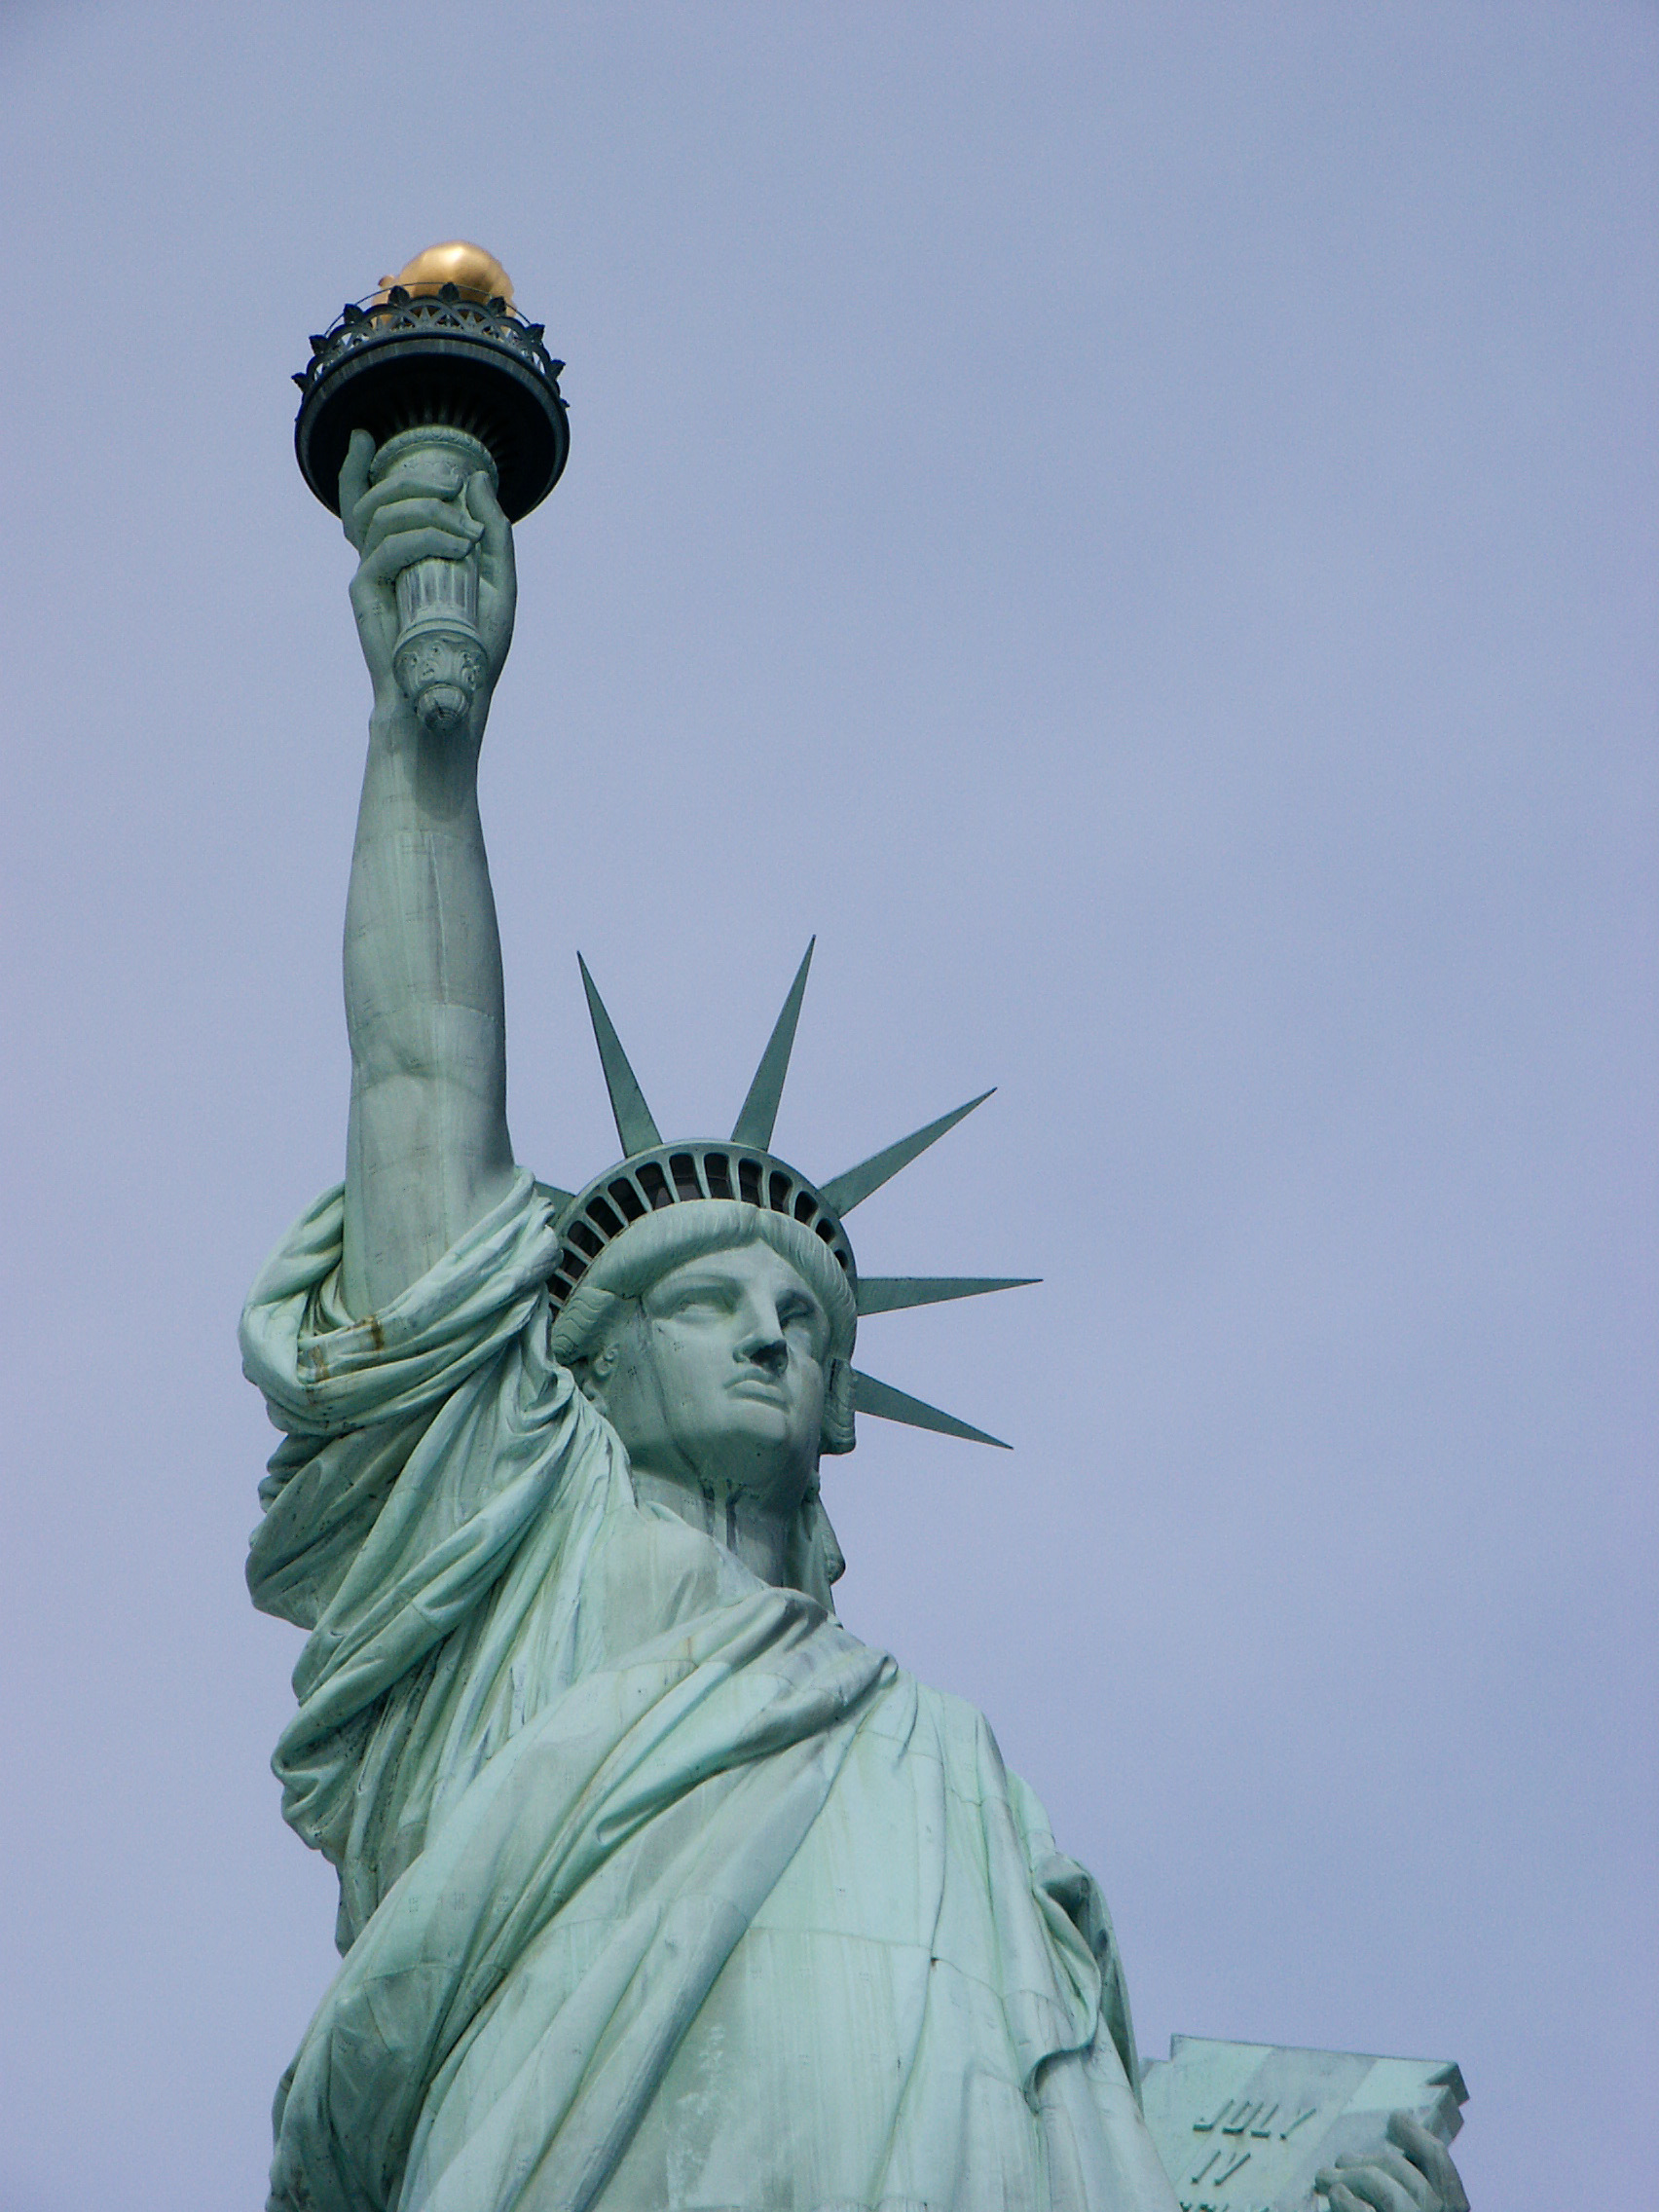
\includegraphics[width=0.25\textwidth]{statue-of-liberty-2-3962082.jpg}}
\label{fig:3720X0}
\end{floatingfigure} Leaving the puppeteers, I made my way to the front entrance of the
building. It was like every visitor center you have ever entered. A fat
black woman with bad breath patted me down and made me run my already
checked camera bags through an x-ray scanner. I picked up my camera bags
and wandered in the Liberty building until I found a dark series of
escalators running up the front of the massive statue. I was suddenly
happy. This must lead to a good viewpoint. I walked up the escalator
steps fumbling with my camera bags. Immediately, in dream steps, I was
at the top of the escalators. They discharged into a small dark brown
room at the very top of Liberty. In the middle of the room, wrapped in
museum display velvet, a bit of Liberty's crown reflected dim halogen
lights. Tourists were touching the exposed crown bit like they kiss the
toes of bronze saints. My movie critic approved, ``This is the way we do
oppression. We don't beat people up; we don't loudly lord it over them;
we don't get in their big fat stupid faces day in and day out. No, we
turn important symbols into tourist attractions, wrap them up as
venerated national monuments, and because we have nasty sense of humor,
we allow well frisked tourists to touch a bit of, `Liberty', while doing
everything we can to deny them real liberty.''

At this point I woke up and thought, ``Boy John, your subconscious
totally nailed it with that one!'' \emph{This is how we do oppression.}
Being a citizen in the \href{http://www.usdebtclock.org/}{Indebted
States of America} is exactly like being a crown touching tourist in my
dream. We pretend the sliver of freedom we're allowed to touch makes us
free but it really only showcases our stupidity and cowardice. A truly
free people would tear down the Liberty encasing visitor center and hang
the architects from the remains of the plane blocking girders.

%\captionsetup[floatingfigure]{labelformat=empty}
%\begin{figure}[htbp]
%\begin{floatingfigure}[l]{0.25\textwidth}
%\centering
%\includegraphics[width=0.23\textwidth]{statue%20of%20liberty%202%20%5B3962082%5D-M.jpg}
%\caption{~~~IMCAPTION~~~}
%\label{fig:3720X0}
%\end{floatingfigure}
%\end{figure}


%\end{document}